\section{The data calculation process}
\begin{enumerate}
    \item logon workstation .(ssh yh@10.249.183.158)
    \item Change program parameters. (Enter (vi run.sh) review the program and change the necessary parameters.)
    \item Enter (make) to determine the changed parameters. 
    \item Start a new process. (screen)
    \item Run the script and output. (./run.sh > output.txt  \&)
    \item Background operation. (Enter(tail -f output.txt) and then obtion the avg.h5 file.) 
\end{enumerate}

\section{data processing}
Enter ./output.py -h to get the program help.

\section{gunplot}
Use gnuplot to draw the figure of the data.
\begin{figure}[htbp]
\centering
    \subfigure{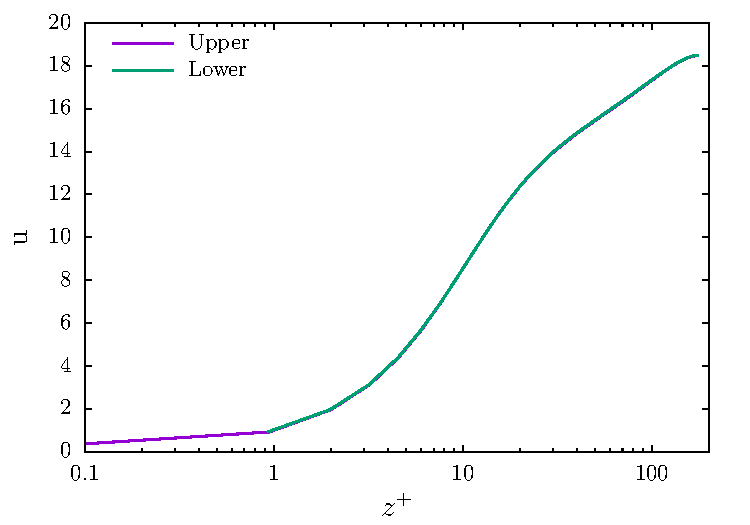
\includegraphics[width=0.35\textwidth]{src/u_sym.pdf}}
 \caption{Mean-velocity profiles:U in wall coordinates,upper wall-purple line,lower wall-green line}
\label{pd}
\end{figure}

\begin{figure}[H]
\centering
    \subfigure{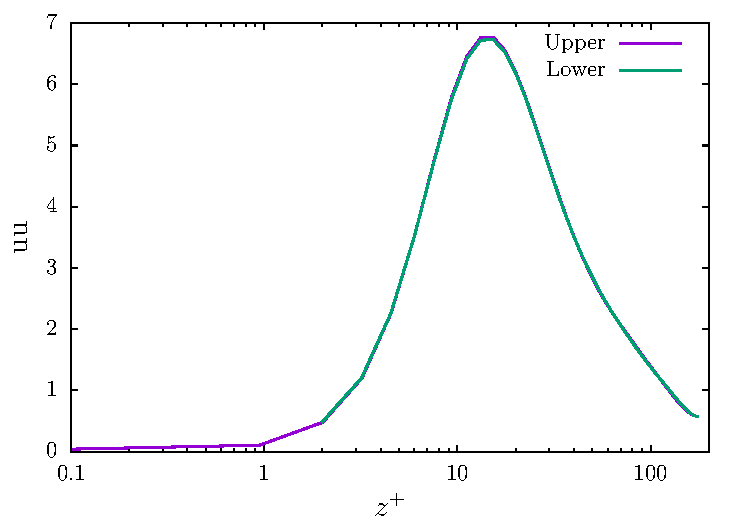
\includegraphics[width=0.35\textwidth]{src/uu_sym.pdf}}
 \caption{Squared velocity fluctuations normalized by the wall shear velocity:u in wall coordinates,upper wall-purple line,lower wall-green line}
\label{pd}
\end{figure}

\begin{figure}[H]
\centering
    \subfigure{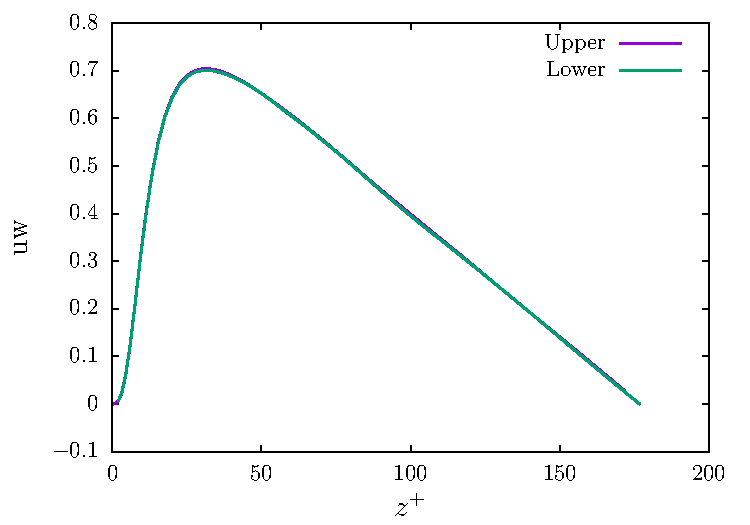
\includegraphics[width=0.35\textwidth]{src/uw_sym.pdf}}
 \caption{Reynolds shear stress normalized by the wall shear velocity in wall coordinates,upper wall-purple line,lower wall-green line}
\label{pd}
\end{figure}

\begin{figure}[H]
\centering
    \subfigure{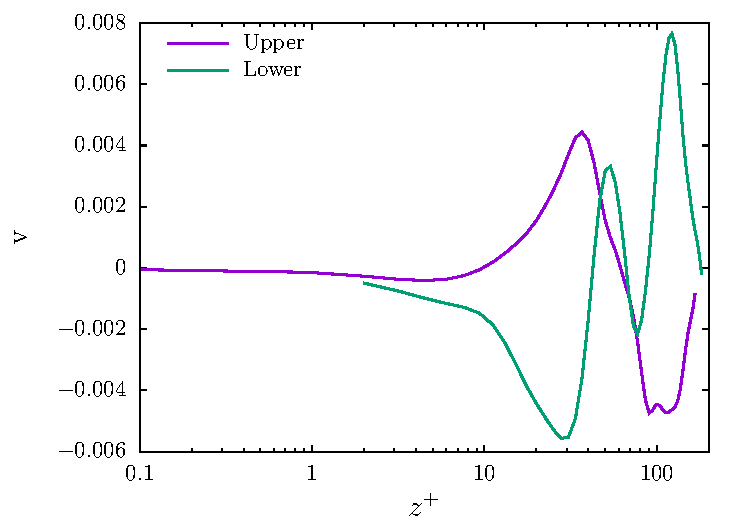
\includegraphics[width=0.35\textwidth]{src/v_sym.pdf}}
 \caption{Mean-velocity profiles:V in wall coordinates,upper wall-purple line,lower wall-green line}
\label{pd}
\end{figure}


\begin{figure}[H]
\centering
    \subfigure{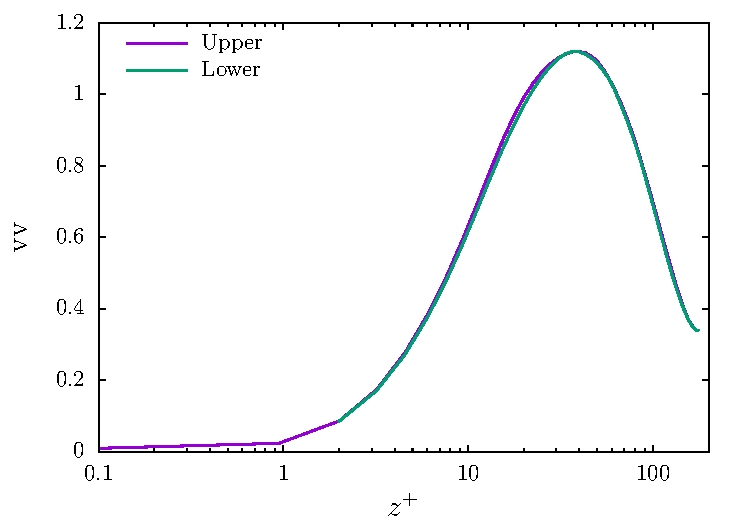
\includegraphics[width=0.35\textwidth]{src/vv_sym.pdf}}
 \caption{Squared velocity fluctuations normalized by the wall shear velocity:v in wall coordinates,upper wall-purple line,lower wall-green line}
\label{pd}
\end{figure}

\begin{figure}[H]
\centering
    \subfigure{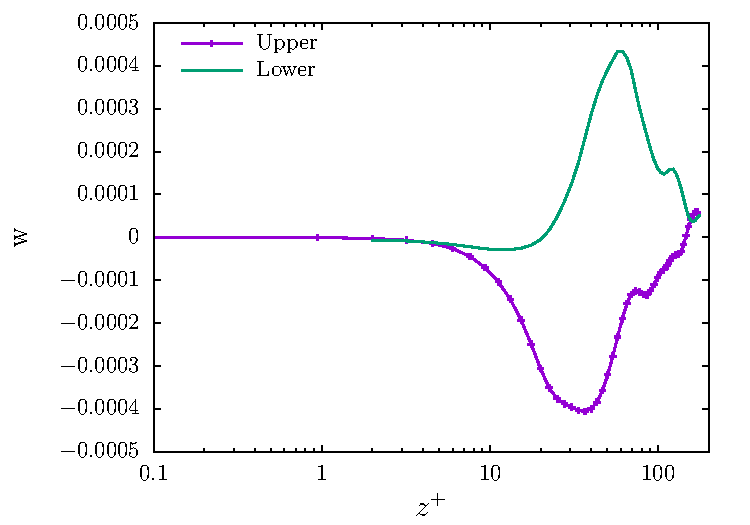
\includegraphics[width=0.35\textwidth]{src/w_sym.pdf}}
 \caption{Mean-velocity profiles:W in wall coordinates,upper wall-purple line,lower wall-green line}
\label{pd}
\end{figure}

\begin{figure}[H]
\centering
    \subfigure{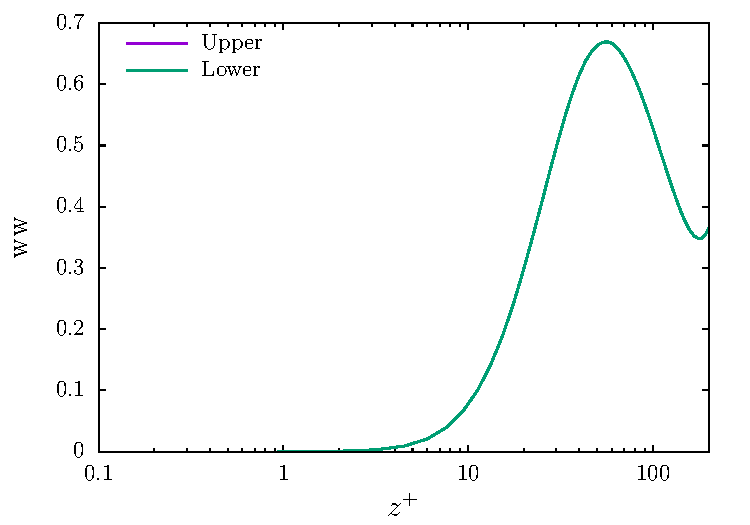
\includegraphics[width=0.35\textwidth]{src/ww_sym.pdf}}
 \caption{Squared velocity fluctuations normalized by the wall shear velocity:w in wall coordinates,upper wall-purple line,lower wall-green line}
\label{pd}
\end{figure}

\begin{figure}[H]
\centering
    \subfigure{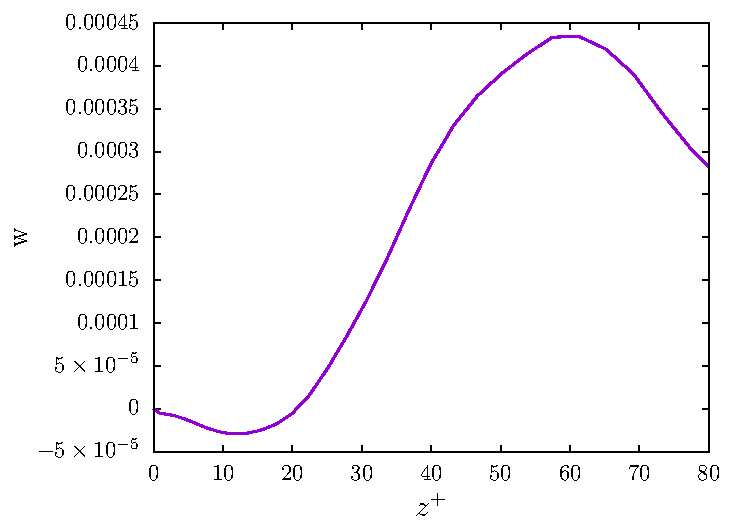
\includegraphics[width=0.35\textwidth]{src/w.pdf}}
 \caption{Mean-velocity profiles:w in wall coordinates,w-puper line}
\label{pd}
\end{figure}

\begin{figure}[H]
\centering
    \subfigure{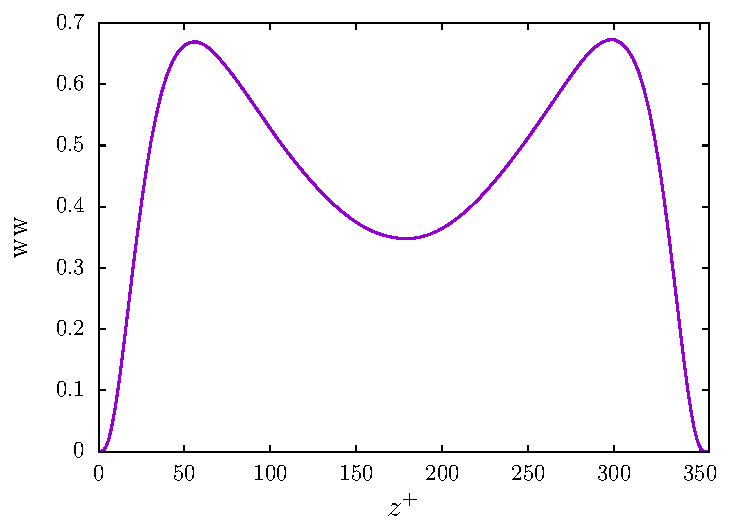
\includegraphics[width=0.35\textwidth]{src/ww.pdf}}
 \caption{Squared velocity fluctuations normalized by the wall shear velocity:w in wall coordinates,ww-puper line}
\label{pd}
\end{figure}

\begin{figure}[H]
\centering
    \subfigure{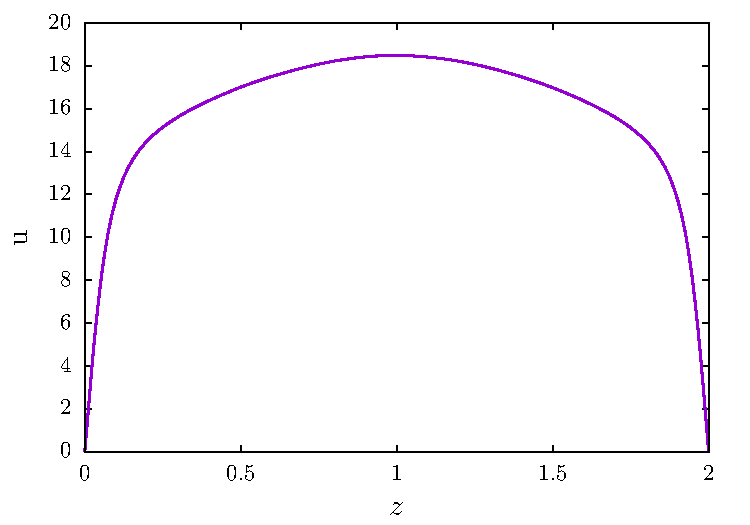
\includegraphics[width=0.35\textwidth]{src/z_u.pdf}}
 \caption{Mean-velocity profiles:U in global coordinates,u-puper line}
\label{pd}
\end{figure}

\begin{figure}[H]
\centering
    \subfigure{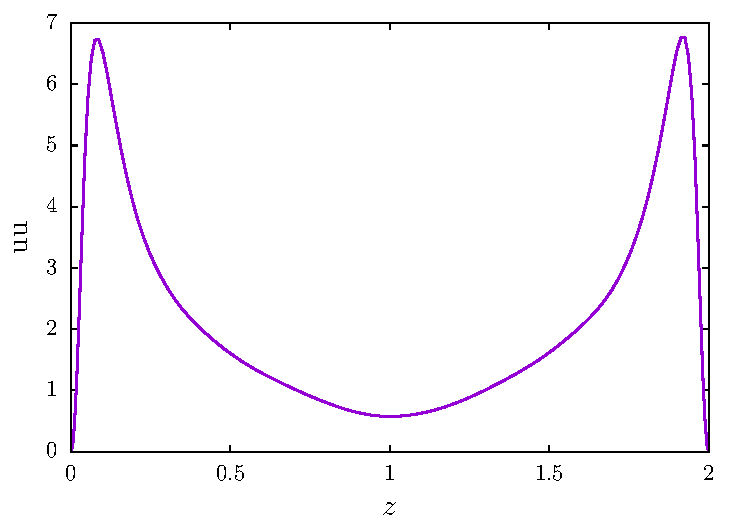
\includegraphics[width=0.35\textwidth]{src/z_uu.pdf}}
 \caption{Squared velocity fluctuations normalized by the wall shear velocity:u in global coordinates,uu-puper line}
\label{pd}
\end{figure}

\begin{figure}[H]
\centering
    \subfigure{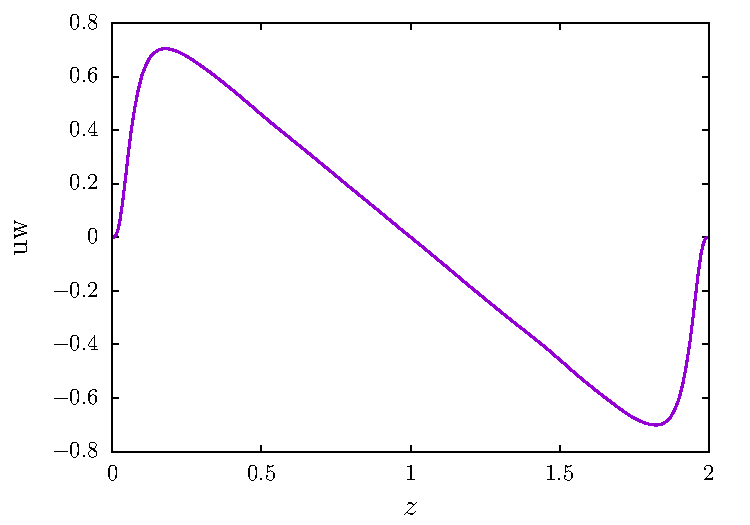
\includegraphics[width=0.35\textwidth]{src/z_uw.pdf}}
 \caption{Reynolds shear stress normalized by the wall shear velocity:in global coordinates,uw-puper line}
\label{pd}
\end{figure}

\begin{figure}[H]
\centering
    \subfigure{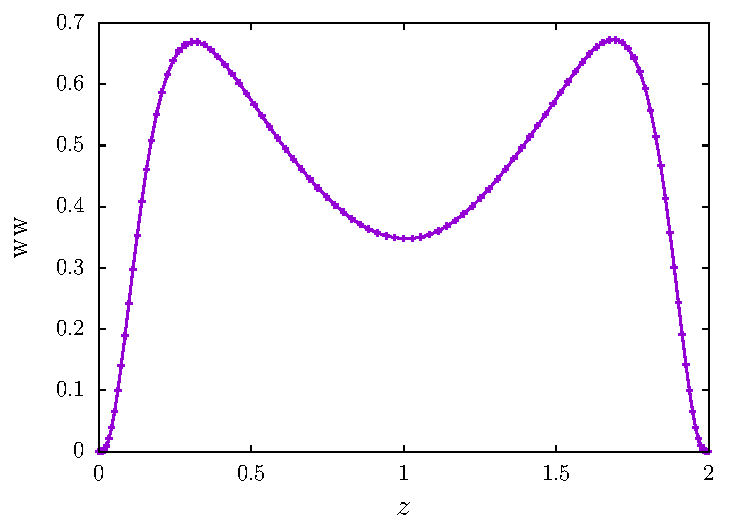
\includegraphics[width=0.35\textwidth]{src/z_ww.pdf}}
 \caption{Squared velocity fluctuations normalized by the wall shear velocity:w in global coordinates,ww-puper line}
\label{pd}
\end{figure}

\vfill




